\section{Marco teórico}

En esta sección se presenta el desarrollo llevado a cabo para lograr los objetivos propuestos, haciendo énfasis en los aspectos teóricos que fundamentan el proyecto.

\subsection{Rectificador de entrada AC-DC}
%Una vez definido el circuito de conversión DC-DC, se procedió a analizar los requisitos de la tensión de entrada. <<< Saqué esto porque queda bastante raro, es recien el principio del capítulo
Los circuitos rectificadores AC-DC permiten convertir una tensión alterna en una tensión continua.
Esta etapa es necesaria para poder entregar una tensión continua al conversor DC-DC.

\subsubsection{Rectificador de media onda u onda completa}

El rectificador de media onda es uno de los circuitos mas simples ya que cuenta solo con un diodo,
por lo que existen muchas ventajas del rectificador de onda completa frente al de media onda.

La primera de ellas es que la corriente media del generador de alterna es nula, lo cual beneficia a los transformadores. 
La segunda se basa en el hecho de que para una misma carga,
la tensión de rizado pico a pico para el rectificador de onda completa es
aproximadamente la mitad que para el rectificador de media onda. 
Esto se debe a que en el circuito de onda completa,
el tiempo durante el que se descarga el capacitor es menor que en el circuito de media onda % Pero acá ya estamos hablando de un filtro
debido a la onda sinusoidal rectificada de la segunda mitad de cada período. 

Por todos estos motivos se decidió implementar un rectificador de onda completa.

\subsubsection{Rectificador de onda completa en puente o con toma media}

El rectificador en puente presenta la caída de tensión de 2 diodos entre el generador y la carga. 
La tensión máxima en un diodo polarizado en inversa es el valor pico del generador.

La variante con transformador de toma media sólo presenta la caída de tensión de un diodo entre el generador y la carga. 
Para una misma potencia entregada por el generador,
los diodos consumen potencia y disminuyen la corriente y potencia que absorbe la carga. 
La tensión máxima en un diodo polarizado en inversa es el doble del valor pico del generador.
El transformador proporciona aislamiento eléctrico entre el generador y la carga. 

Como la reducción de tensión a la salida no es significativa en esta aplicación
y el puente de diodos se puede implementar con un pequeño integrado,
con el objetivo de disminuir el tamaño del circuito se decidió evitar el transformador
y utilizar un rectificador de onda completa tipo puente.

\subsubsection{Rectificación controlada}

La rectificación controlada es un método que utiliza tiristores y permite controlar el ángulo de conmutación de la tensión de salida.
Los tiristores son interruptores electrónicos controlados que son activados por una señal externa. 
Poseen 3 terminales: ánodo, cátodo y puerta. Presentan altos valores nominales de corriente y tensión.
Soportan altas corrientes y altas tensiones de bloqueo. 

Un ejemplo de tiristores con los rectificadores controlados de silicio (SCR).
Para que conduzcan se los debe polarizar en directa y deben recibir una corriente de puerta. 
Al entrar en conducción no es necesaria la señal de puerta para mantener la corriente de ánodo. 
El SCR continuará conduciendo siempre que la corriente de ánodo sea positiva y esté por arriba de un valor mínimo. 

Mediante conmutadores controlados como los SCR se controla la tensión de salida en un rango limitado de variación, ajustando el ángulo de disparo de cada SCR. 
El ángulo de disparo es el intervalo angular entre la polarización directa del SCR y la aplicación de la señal de puerta. 
Si el ángulo de disparo es 0, el comportamiento es igual al de un rectificador no controlado con diodos. 

Se decidió utilizar rectificación no controlada ya que no se necesita una tensión específica a la salida
y el costo de complejizar el diseño con el agregado de SCRs y un circuito dedicado de disparo no aporta ningún beneficio significativo.

\subsubsection{Filtrado}

El filtro pasa bajos compuesto por una red LC permite disminuir el rizado,
es decir, la componente de alterna de la señal rectificada. 
Como resultado se logra una tensión de salida aproximadamente continua.
El capacitor mantiene la tensión de salida en un nivel constante y
la bobina suaviza la corriente del rectificador y reduce la corriente de pico en los diodos. 

Para disminuir el número de componentes se decidió utilizar únicamente
un capacitor en paralelo con la capacidad suficiente para obtener una tensión continua.

\subsection{Fuentes de alimentación}

Las fuentes de alimentación otorgan una alta densidad de potencia en un tamaño mediano y con un peso reducido.  
Permiten aislar eléctricamente a la carga de la red de alimentación con una alta eficiencia de conversión.
Utilizando filtros simples es posible tener formas de onda con baja distorsión armónica tanto en la entrada como en la salida. 
Para poder utilizar un transformador pequeño y cumplir con las especificaciones normalmente se requieren múltiples etapas de conversión. 
En base a la tensión de salida requerida existen fuentes de alimentación AC y fuentes de alimentación DC.
Dado el requisito de tensión de salida de continua, se debe diseñar una fuente de alimentación DC, las cuales se clasifican en:

\paragraph{Conmutadas}
Tienen una alta eficiencia y pueden suministrar altas corrientes de carga a una tensión baja.
Existen 5 topologías comunes: fly-back, forward, push–pull, half-bridge, y full-bridge.
Por lo general se utilizan 2 etapas de conversión: DC-AC mediante modulación de ancho de pulso (PWM) y de AC-DC.
La salida del inversor, que varía mediante una señal PWM, se convierte en un voltaje DC mediante un rectificador de diodos. 
Debido a que el inversor puede operar a una frecuencia muy alta, las fluctuaciones en la tensión de salida de DC se pueden filtrar fácilmente.

\paragraph{Resonantes}
Si la variación del voltaje de salida no es amplia se pueden usar inversores de pulso resonante. 
La frecuencia del inversor, que podría ser la misma que la frecuencia de resonancia, es muy alta y la tensión de salida del inversor es casi sinusoidal.
Debido a la oscilación resonante, el núcleo del transformador siempre se restablece y no hay problemas de saturación. 
Los tamaños del transformador y del filtro de salida se reducen debido a la alta frecuencia del inversor.

\paragraph{Bidireccionales}
Aptas para carga y descarga de baterías donde el flujo de potencia es bidireccional.
Este último depende de la tensión de entrada, de la tensión de salida y de la relación de vueltas del transformador. 
Permiten que la corriente inductiva fluya en cualquier dirección y que el flujo de corriente se vuelva continuo.
Requiere sintetizar las funciones de conmutación para obtener las formas de onda de salida deseadas.\\

Dado que no se requiere de un flujo de potencia bidireccional en la carga de las baterías y la mayor complejidad de las fuentes resonantes, 
se optó por desarrollar una fuente de alimentación conmutada. 

\subsection{Elección del convertidor}

El primer paso de diseño fue la elección de una topología de conversión DC-DC.
Para seleccionar una topología adecuada es necesario analizar los requisitos de la aplicación y las ventajas y desventajas de cada topología.  
Sólo se describe de forma completa la topología utilizada en el proyecto. En cuanto a las restantes, se detallarán los motivos que llevaron a su exclusión.  

El convertidor introduce aislación a partir de un transformador de alta frecuencia,
disminuyendo el coste, tamaño y peso respecto a uno de baja frecuencia en base al núcleo magnético necesario.
Como se requiere una única tensión de salida no se utilizan múltiples devanados.

Aunque la mayor parte de los convertidores se pueden utilizar para cumplir con los requerimientos de salida, 
los valores nominales del dispositivo de conmutación y el tamaño del transformador limitan sus aplicaciones a una potencia de salida específica. 
Por lo tanto, la elección del convertidor depende del requisito de potencia de salida y de la complejidad que se desea afrontar.
Para el cargador de baterías, el convertidor debe alcanzar una potencia máxima de 300W y debe ser lo más sencillo posible para evitar un costo elevado. 

La topología flyback es de baja complejidad al estar integrada por muy pocos componentes. 
Como desventajas, el tamaño del núcleo del transformador se incrementa con la potencia requerida y en bornes del
interruptor presenta una tensión igual al doble de la tensión máxima de entrada.
En aplicaciones típicas se alcanzan valores de hasta 150W.

La topología forward con un solo switch disminuye el tamaño del núcleo del transformador ya que la energía no necesita almacenarse en el entrehierro.
Como desventajas, al igual que el flyback presenta alta tensión en bornes del interruptor y se eleva el costo debido al agregado de la bobina de filtrado.
La topología forward con dos switches reduce la tensión en bornes del interruptor a la mitad respecto a la de un solo switch (y con ello la disipación de potencia por switch), 
pero el circuito de excitación de uno de los transistores queda flotante respecto a masa. 
La topología con un solo switch admite una potencia de salida entre 150-250W y con 2 switches se eleva a 750W \cite{mohan}\cite{hart}. 
Por lo tanto, en base a los criterios definidos inicialmente se eligió al convertidor forward con dos switches como topología de conversión DC-DC. 

\subsubsection{Convertidor Forward}

Es un convertidor DC-DC acoplado magnéticamente. El transistor funciona como interruptor, estará cerrado un tiempo $DT$ y abierto el resto del tiempo,
$(1 - D)T$, siendo $T$ el periodo de conmutación. 
El transformador posee tres devanados: los devanados 1 y 2 transfieren la energía de la
fuente a la carga cuando el interruptor está cerrado; el devanado 3 se usa para proporcionar un
camino a la corriente magnetizante cuando el interruptor está abierto y reducirla a cero antes del
inicio de cada periodo de conmutación. El transformador se modela como tres devanados ideales
con una inductancia magnetizante $L_m$ conectada en paralelo con el devanado 1. En este modelo simplificado no se incluyen las pérdidas ni las inductancias de dispersión.
En el convertidor forward, $L_m$ es un parámetro no incluido en la relación entrada-salida y se suele adoptar un valor grande.
En la figura \ref{fig:conversor_forward} se muestra el esquema del convertidor con un solo switch.

\begin{figure}[ht]
    \centering
    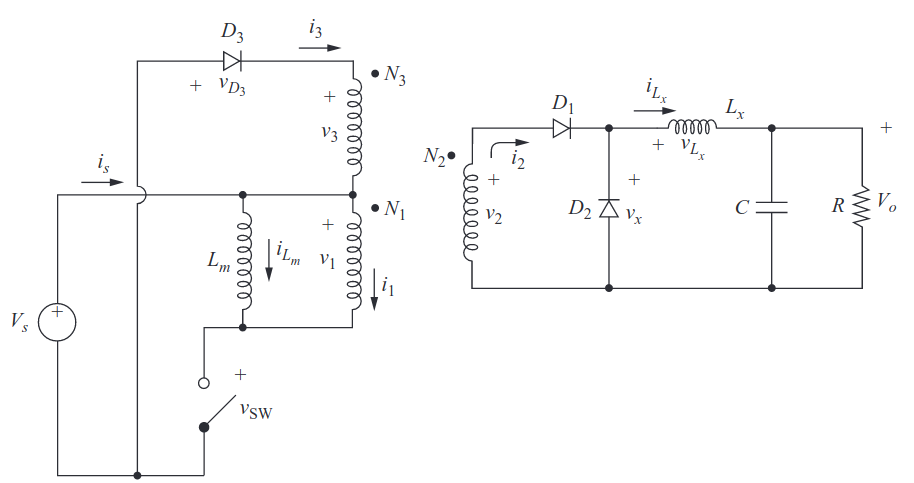
\includegraphics[width=0.8\textwidth]{../images/hart/conversor_forward.png}
    \caption{Esquema del convertidor forward de un solo switch}
    \label{fig:conversor_forward}
\end{figure}

% No se si está bueno comparar con otro conversor antes de explicarlo
% A diferencia del convertidor flyback, la energía del generador se transfiere a la carga cuando el interruptor
% está cerrado. En el convertidor flyback, la energía se almacena en el primario cuando el conmutador
% está cerrado y se transfiere a la carga cuando está abierto. 
En esta topología, la energía del generador se transfiere a la carga cuando el interruptor está cerrado.
Esto lo diferencia del convertidor flyback, en el cual la energía se almacena en el primario cuando el conmutador está cerrado y se transfiere a la carga cuando está abierto.

La eficiencia se incrementa reestableciendo el núcleo del transformador,
ya que la energía almacenada en el mismo es devuelta a la fuente de entrada del convertidor a partir del tercer bobinado. 
Además, sólo se opera en el modo de conducción continua por la mayor dificultad del control en base al doble polo existente en el filtro de salida. 

% REVISAR NOMENCLATURA EN BASE A LAS IMÁGENES A UTILIZAR DE LOS LIBROS
Asumiendo modo de conducción continua, operación en estado estacionario, ripple de salida nulo 
y que la corriente en la inductancia del filtro de salida $L_x$ es permanente, existen 2 modos de operación del transistor:

% RASHID EN INGLÉS

\paragraph{Cuando el transistor se encuentra encendido}

En la figura \ref{fig:forward_switch_closed} se muestra el circuito equivalente del convertidor forward cuando el interruptor
está cerrado. Al cerrarse el interruptor se establece una tensión en el primer devanado del transformador,
lo cual induce tensiones en el segundo y tercer devanado:

% HART INGLÉS PÁGINA 279 DEL LIBRO 
$$ v_1=V_s $$
$$ v_2=v_1\left(\frac{N_2}{N_1}\right)=V_s\left(\frac{N_2}{N_1}\right) $$
$$ v_3=v_1\left(\frac{N_3}{N_1}\right)=V_s\left(\frac{N_3}{N_1}\right) $$

\begin{figure}[ht]
    \centering
    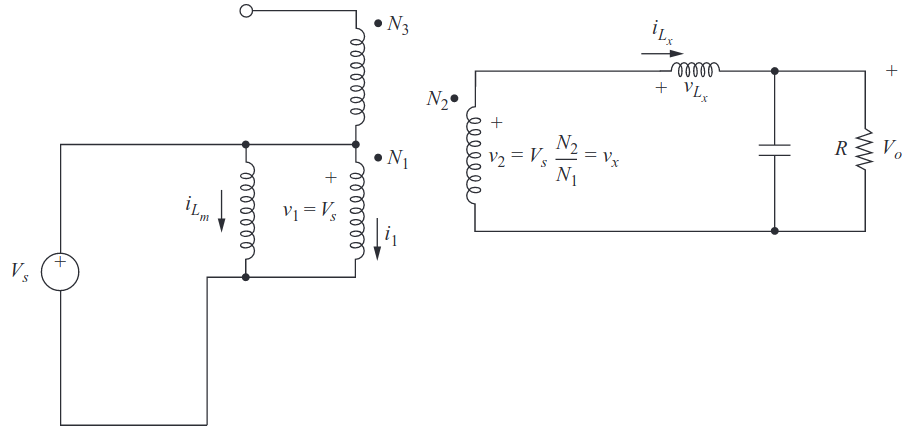
\includegraphics[width=0.8\textwidth]{../images/hart/forward_switch_closed.png}
    \caption{Convertidor forward cuando el interruptor está cerrado}
    \label{fig:forward_switch_closed}
\end{figure}

La tensión $v_2$ positiva polariza en directa a $D_1$ y en reversa a $D_2$. El diodo $D_3$ no conduce ya que su tensión es negativa:

$$ V_{D_3}=-V_s-v_3<0 $$

La tensión en la bobina es:
% vlx
$$ v_{L_x}=v_2-V_0=V_s\left(\frac{N_2}{N_1}\right)-V_o=L_x\frac{di_{L_x}}{dt} $$

Reorganizando los términos obtenemos:
% ecuación de abajo
$$ \frac{di_{L_x}}{dt}=\frac{V_s(N_2/N_1)-V_o}{L_x}=\frac{\Delta i_{L_x}}{\Delta t}=\frac{\Delta i_{L_x}}{DT} $$

Como la derivada de la corriente es una constante positiva, la corriente aumenta linealmente. 
La variación de corriente cuando el interruptor está cerrado se calcula modificando la ecuación anterior:
% ecuación de abajo 7-22
$$ (\Delta i_{L_x})_{closed}=\left[V_s\left(\frac{N_2}{N_1}\right)-V_o\right]\frac{DT}{L_x} $$

La tensión en la inductancia magnetizante es igual a la tensión en el primario del transformador, por lo cual:
% ecuación 7-23
$$ \Delta i_{L_m}=\frac{V_sDT}{L_m} $$

La corriente que circula por el transistor está compuesta por:
% ecuación 7-24
$$ i_{sw}=i_1+i_{L_m} $$

% FIN HART INGLÉS PÁGINA 279 DEL LIBRO

La corriente que circula por el primario comienza a incrementarse,
se transfiere energía del primario al secundario y de aquí al filtro de salida y la carga por medio del diodo $D_2$ polarizado en directa. 
Debido a esta corriente se induce una corriente en el secundario dada por:
% RASHID INGLÉS PÁGINA 666 DEL LIBRO 
$$ i_p=\frac{N_s}{N_p}i_{se} $$

Por lo tanto, 
% ESCRIBIR iprimario=f(isecundario)  (al reves que antes)
$$ i_p=f(i_{se}) $$

La corriente magnetizante se incrementa linealmente con el tiempo:

$$ i_{mag}=\frac{V_s}{L_m}t $$

La corriente total que circula por el primario resulta:

$$ i_p'=i_p+i_{mag}=\frac{N_s}{N_p}i_{se}+\frac{V_s}{L_m}t $$

Cuando finaliza el tiempo de conducción del transistor en un tiempo $t=DT$, esta corriente llega a un valor máximo dado por:

$$ I_{p_{max}}'=I_{p_{max}}+\frac{V_sDT}{L_m} $$

donde $I_{p_{max}}$ es la corriente pico reflejada a la salida del inductor $L_x$ y está dada por:

$$ I_{p_{max}}=\frac{N_p}{N_s}I_{L_{1_{max}}} $$

Debido a la tensión $V_{se}-V_o$ existente en bornes del inductor de salida, su corriente se incrementa linealmente:

$$ \frac{di_{L_x}}{dt}=\frac{V_s-V_o}{L_x} $$

Esta misma también tendrá su valor máximo en $t=DT$:

$$ I_{L_{1_{max}}}=I_{L_x}(0)+\frac{(V_s-V_o)DT}{L_x} $$

\paragraph{Cuando el transistor se encuentra apagado}
En la figura \ref{fig:forward_switch_open} se muestra el circuito equivalente del convertidor forward cuando el interruptor está abierto. 
Las tensiones de todos los bobinados del transformador toman polaridad negativa, lo cual apaga al diodo $D_1$ y enciende a los diodos $D_2$ y $D_3$. 
La corriente magnetizante y la corriente en el inductor del filtro de salida no pueden cambiar instantáneamente cuando el transistor se apaga. 
La continuidad de $i_{L_m}$ establece $ i_1=-i_{L_m} $
% SACAR DEL TEXTO INICIAL

\begin{figure}[ht]
    \centering
    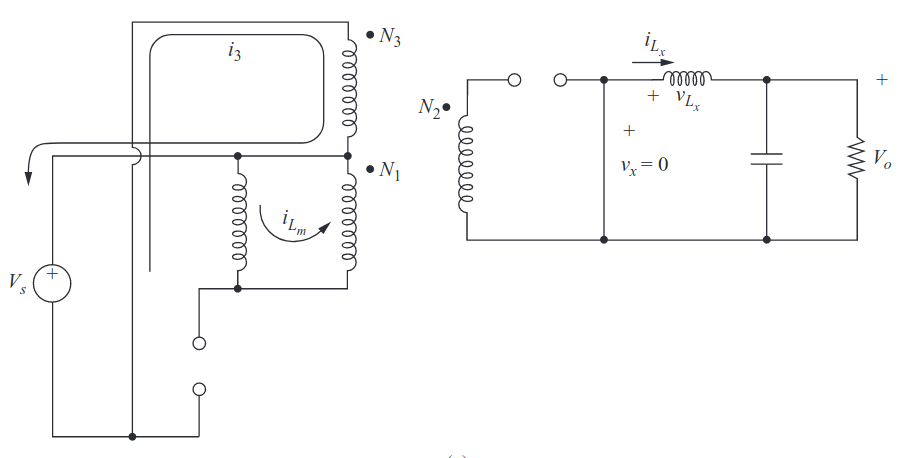
\includegraphics[width=0.8\textwidth]{../images/hart/forward_switch_open.png}
    \caption{Convertidor forward cuando el interruptor está abierto}
    \label{fig:forward_switch_open}
\end{figure}

La corriente que sale del terminal con punto homólogo del primer bobinado quiere establecer una corriente que ingresa al terminal 
con punto homólogo del segundo bobinado, pero el diodo $D_1$ no permite la circulación de la corriente en esa dirección. 
Además, la corriente que sale del terminal con punto homólogo del primer bobinado induce una corriente que ingresa al terminal 
con punto homólogo del tercer bobinado. Esto polariza en directa al diodo $D_3$, a la vez que 
se le provee a la corriente magnetizante de un camino a través del tercer bobinado de regreso a la fuente de entrada. 

Con $D_3$ encendido, la tensión en el tercer bobinado resulta:
% HART EN INGLES PÁGINA 280 DEL LIBRO 
$$ v_3=-V_s $$

Esto induce las siguientes tensiones en los otros bobinados:
% ECUACIÓN 7.25
$$ v_1=v_3\left(\frac{N_1}{N_3}\right)=-V_s\left(\frac{N_1}{N_3}\right) $$
$$ v_2=v_3\left(\frac{N_2}{N_3}\right)=-V_s\left(\frac{N_2}{N_3}\right) $$

Con $D_1$ apagado y corriente positiva en el inductor de salida, $D_2$ se polariza en directa. 
Mientras conduce $D_2$, la energía es entregada a la carga a través del inductor de salida. 
La tensión sobre la misma resulta:
% ECUACIÓN 7.26
$$ v_{L_x}=-V_o=L_x\frac{di_{L_x}}{dt} $$

Reorganizando los términos obtenemos:

$$ \frac{di_{L_x}}{dt}=\frac{V_o}{L} $$

Como la derivada de la corriente es una constante negativa, la corriente disminuye linealmente. 
La variación de corriente cuando el interruptor está abierto se calcula modificando la ecuación anterior:

$$ (\Delta i_{L_x})_{open}=\frac{-V_o(1-D)T}{L_x} $$

La corriente por el inductor y el diodo $D_2$ es la misma y decrece linealmente con el tiempo:
%% RASHID (13.19)
$$ i_{L_x}=i_{D_3}=I_{L_{x_{max}}}-\frac{V_o}{L_x}t,\ 0<t\leq (1-k)T $$

Lo cual nos da el valor de $I_L(t=0)=i_{L_x}(t=(1-k)T)=I_{L_{x_{max}}}-V_o(1-k)T/L_x$
%% RASHID POST (13.19)

En estado estacionario el cambio neto en la corriente del inductor durante un período debe ser cero:
% ECUACIÓNES PRE 7.27
$$ (\Delta i_{L_x})_{closed}+(\Delta i_{L_x})_{open}=0 $$
$$ \left[V_s\left(\frac{N_2}{N_1}\right)-V_o\right]\frac{DT}{L_x}-\frac{V_o(1-D)T}{L_x}=0 $$

Resolviendo se obtiene la tensión de salida:
% ECUACIÓN 7.27
$$ V_o=V_sD\left(\frac{N_2}{N_1}\right) $$

La tensión en la inductancia magnetizante es igual a la tensión en el primario del transformador, la cual decrece linealmente con el tiempo:
% ECUACIÓN 7.28 Y 7.29
$$ v_{L_m}=v_1=-V_s\left(\frac{N_1}{N_3}\right)=L_m\frac{di_{L_m}}{dt} $$

$$ \frac{di_{L_m}}{dt}=-\frac{V_s}{L_m}\left(\frac{N_1}{N_3}\right) $$

$$ \frac{\Delta i_{L_m}}{\Delta t}=-\frac{V_s}{L_m}\left(\frac{N_1}{N_3}\right) $$ 

Se puede observar que el diodo $D_3$ impide que la corriente $i_{L_m}$ se haga negativa. 

% VER DONDE PONER ESTAS 2 ECUACIONES
%% RASHID (13.21) Y (13.22)
La máxima corriente de colector se da durante el encendido del transistor y la máxima tensión de colector durante el apagado:

$$ I_{C_{max}}=I_{p_{max}}'=\left(\frac{N_p}{N_s}\right)I_{L_{x_{max}}}+\frac{V_sDT}{L_m} $$
$$ V_{Q_{1_{max}}}=V_{s_{max}}+V_{r_{max}}=V_{s_{max}}\left(1+\frac{N_p}{N_r}\right) $$

Para que el flujo magnético vuelva a 0, la corriente magnetizante debe anularse al final de cada ciclo de conmutación, desmagnetizando el núcleo del transformador.
Para lograrlo, el decrecimiento de la corriente debe ser igual a su incremento dado por la variación de corriente cuando el interruptor está cerrado. 
Si el tiempo necesario para que la corriente $i_{L_m}$ se anule desde su valor máximo es $\Delta T_x$, 
% ECUACIÓN 7.30
$$ \frac{\Delta i_{L_m}}{\Delta T_x}=-\frac{V_sDT}{L_m}=-\frac{V_s}{L_m}\left(\frac{N_1}{N_3}\right) $$

Resolviendo para obtener $\Delta T_x$,
% ECUACIÓN 7.31
$$ \Delta T_x=DT\left(\frac{N_3}{N_1}\right) $$

El instante $t_0$ en el que se anula la corriente es:
% ECUACIÓN 7.32
$$ t_0=DT+\Delta T_x=DT+DT\left(\frac{N_3}{N_1}\right)=DT\left(1+\frac{N_3}{N_1}\right) $$

Teniendo en cuenta que la corriente debe anularse antes del inicio del siguiente periodo,
% ECUACIÓN 7.33
$t_0<T$

$$ sDT\left(1+\frac{N_3}{N_1}\right)<T $$

$$ D\left(1+\frac{N_3}{N_1}\right)<1 $$

Para evitar la saturación del núcleo del transformador, el ciclo de trabajo debe mantenerse siempre por debajo del máximo.
El transistor puede dañarse si el núcleo se satura.

La tensión en el interruptor abierto es $V_s-v_1$, por lo que
% ECUACIÓN 7.34
$$
v_{sw}=
\begin{cases}
    V_s-v_1=V_s-\left(-V_s\frac{N_1}{N_3}\right)=V_s\left(1+\frac{N_1}{N_3}\right) & \text{para $DT<t<t_0$}\\
    V_s & \text{para $t_0<t<T$}
\end{cases}
$$

% FIN HART EN ESPAÑOL PÁG 272

% HART EN ESPAÑOL PÁG 208

En el análisis anterior hemos supuesto ripple de salida nulo, es decir, que el capacitor de salida era muy grande para que la tensión
de salida fuese constante. En la práctica no será posible mantener perfectamente constante la
tensión de salida con una capacidad finita. La variación periódica de la tensión de salida, o rizado,
se calcula a partir de la relación entre la tensión y la corriente del capacitor. 
La corriente en el capacitor es:

$$ i_C=i_L-i_R $$

Dicha corriente se muestra en la figura \ref{fig:buck_converter_capacitor_current}.
El capacitor se cargará mientras sea positiva la corriente en el mismo. Aplicando la definición de capacidad,

$$ Q=CV_o $$

$$ \Delta Q=C\Delta V_o $$

$$ \Delta V_o=\frac{\Delta Q}{C} $$

\begin{figure}[ht]
    \centering
    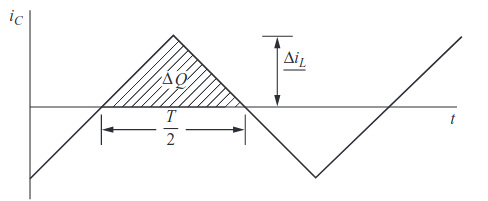
\includegraphics[width=0.8\textwidth]{../images/hart/buck_converter_capacitor_current.png}
    \caption{Corriente por el capacitor de salida}
    \label{fig:buck_converter_capacitor_current}
\end{figure}

La variación de la carga, $\Delta Q$, es el área del triángulo situado por encima del eje de tiempos:

$$ \Delta Q=\frac{1}{2}\left(\frac{T}{2}\right)\left(\frac{\Delta i_L}{2}\right)=\frac{T\Delta i_L}{8} $$

Reemplazando:

$$ \Delta V_o=\frac{T\Delta i_L}{8C} $$

Sustituyendo el valor de la variación de corriente en la bobina cuando el interruptor está abierto, 
se obtiene la tensión de rizado pico a pico en la salida, mostrada en la figura \ref{fig:buck_converter_capacitor_ripple_voltage}.

$$ \Delta V_o=\frac{T}{8C}\frac{V_o}{L}(1-D)T=\frac{V_o(1-D)}{8LCf^2} $$

\begin{figure}[ht]
    \centering
    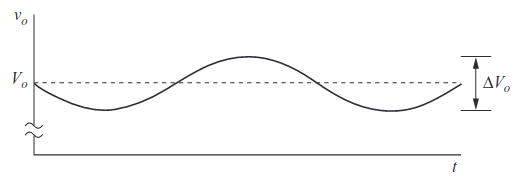
\includegraphics[width=0.8\textwidth]{../images/hart/buck_converter_capacitor_ripple_voltage.png}
    \caption{Tensión de rizado pico a pico a la salida}
    \label{fig:buck_converter_capacitor_ripple_voltage}
\end{figure}

Si el rizado no es muy grande, la suposición de que la salida es constante es razonable, y el
análisis anterior será válido.

% FIN HART EN ESPAÑOL PÁG 209

En resumen, cuando el interruptor está cerrado, la fuente entrega energía a la carga a través del transformador.
La tensión en el secundario del transformador es una forma de onda pulsante. La energía almacenada en
la inductancia magnetizante cuando el interruptor está cerrado es devuelta a la fuente de
entrada a través de un tercer devanado del transformador cuando el interruptor está abierto.

En comparación con el convertidor flyback, el convertidor forward requiere de una carga mínima para evitar un exceso en la tensión de salida. 
Como el transformador no almacena energía, para un mismo nivel de potencia de salida, 
el tamaño del mismo es menor en el convertidor forward que en el flyback. 
Además, la corriente de salida es aproximadamente constante ya que el ripple disminuye notablemente 
debido al agregado del inductor en la salida y al diodo de rueda libre $D_1$.
Por esto mismo, el capacitor de salida puede ser más pequeño. 

\subsubsection{Convertidor Forward Doble Switch}

El convertidor forward se utiliza para potencias de salida de hasta 200W ya que se encuentra limitado 
por los esfuerzos de tensión y corriente a los que se somete el transistor de potencia durante su funcionamiento. 
El convertidor forward de doble switch puede ser utilizado con potencias de hasta 750W \cite{mohan}.
En la figura \ref{fig:forward_doble_switch} se muestra el esquema de éste último.
A partir de los diodos $D_3$ y $D_4$ en el primario, se reduce la tensión de colector en los transistores cuando los mismos 
se encuentran apagados, lo cual permite utilizar transistores de menores prestaciones.

\begin{figure}[ht]
    \centering
    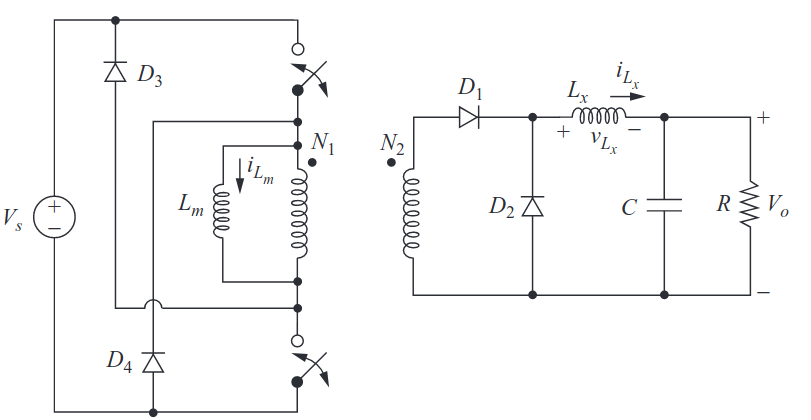
\includegraphics[width=0.8\textwidth]{../images/hart/forward_doble_switch.png}
    \caption{Esquema del convertidor forward de doble switch}
    \label{fig:forward_doble_switch}
\end{figure}

Los transistores se encienden y se apagan de forma simultánea, lo cual los diferencia de las topologías bridge. 
Cuando los transistores están encendidos, la tensión en el primario del transformador es igual a la tensión de entrada $V_s$. 
En consecuencia, la tensión en el devanado secundario es positiva y la energía se transfiere a la carga. 
Además la corriente que circula por la inductancia magnetizante se incrementa con el tiempo. 

Cuando los transistores se apagan, el diodo $D_1$ evita que la corriente magnetizante circule por el secundario 
(y por lo tanto también en el primario) del transformador, forzando su camino por los diodos $D_3$ y $D_4$ de regreso a la fuente de entrada.  
Con esto se elimina la necesidad del tercer devanado de desmagnetización. 
La tensión en el primario del transformador es $-V_s$, causando un decremento en el tiempo de la corriente magnetizante. 
Si la relación de trabajo de los transistores es menor a 0.5, en cada ciclo el núcleo del transformador se restablece.
La tensión de salida es la misma que la del convertidor forward con un interruptor descrito anteriormente.
La principal ventaja de esta topología es que la tensión de colector en los transistores cuando los mismos se encuentran apagados 
es $V_s$ y no $V_s\left(1+N_1/N_3\right)$ como en el forward de un único switch.

\subsection{Circuitos de control}

La tensión de salida del convertidor puede ser controlada variando el ciclo de trabajo D. 
Para ello se utilizan circuitos integrados controladores PWM que sólo requieren de unos pocos componentes pasivos adicionales para su funcionamiento. 
Internamente presenta 4 componentes principales:
\begin{enumerate}
    \item Un reloj ajustable que permite configurar la frecuencia de conmutación
    \item Amplificador de error para la tensión de salida
    \item Generador de forma de onda de dientes de sierra sincronizado con el reloj
    \item Un comparador para comparar la señal de salida de error con la señal de dientes de sierra
\end{enumerate}

La señal de salida del circuito PWM es la que controla a los transistores. 
Para controlar la tensión de salida, los convertidores funcionan con un circuito de retroalimentación,
dependiendo de la señal realimentada, en un control por tensión o corriente. En la figura \ref{fig:marco_teorico:control} se muestra un diagrama de bloques del circuito.

\begin{figure}[ht]
    \centering
    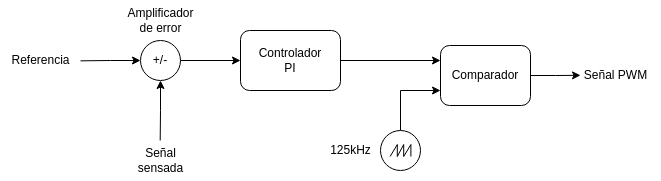
\includegraphics[width=0.8\textwidth]{images/compensador.png}
    \caption{Diagrama de bloques del circuito de control}
    \label{fig:marco_teorico:control}
\end{figure}

\subsubsection{Control por tensión}

%COMPLETAR CON LIBRO
El bloque de control mide la tensión a la salida del convertidor, la escala y la compara con la tensión deseada.
Esto genera una señal de error, la cual alimenta a un controlador PI.

La duración del tiempo de encendido está determinada por el tiempo entre el reinicio del generador de diente de sierra
y la intersección del voltaje de error con la señal de rampa positiva. 
Cuando la tensión de salida es inferior al valor nominal se genera una tensión de error. 
El ciclo de trabajo aumenta para causar un aumento posterior en el voltaje de salida. 
%La dinámica de retroalimentación está determinada por el circuito amplificador de error que consta de Z1 y Z2.

\subsubsection{Control por corriente}
La corriente a la salida del conversor es medida con una resistencia de bajo valor conectada en serie con la carga.
Esta resistencia actúa como un transductor de corriente a tensión, por lo que ambos métodos de control son similares.

% Consiste en un lazo interno que muestrea el valor de la corriente primaria y apaga los interruptores tan pronto como la corriente alcanza cierto valor establecido por el lazo de voltaje externo. 
% De esta manera, el control de corriente logra una respuesta más rápida que el modo de voltaje. 
% La forma de onda de corriente primaria actúa como onda de diente de sierra. 
% la tensión análoga a la corriente puede ser proporcionada por una pequeña resistencia o por un transformador de corriente. 
% La figura 13.19a muestra un convertidor flyback controlado por modo de corriente, donde la corriente del interruptor isw se usa como señal portadora. 
% La corriente del interruptor isw produce un voltaje a través de Rs, que se retroalimenta al comparador. 
% El encendido está sincronizado con el pulso del reloj y el apagado está determinado por el instante en que la corriente de entrada es igual al voltaje de error.
% Debido a su capacidad inherente de limitación de corriente máxima, el control de modo de corriente puede mejorar la confiabilidad de los interruptores de alimentación. El rendimiento dinámico se mejora debido al uso de la información actual adicional. El control de modo de corriente reduce efectivamente el sistema a primer orden al obligar a que la corriente del inductor se relacione con el voltaje de salida, logrando así una respuesta más rápida. Las figuras 13.18b–e muestran las formas de onda.

% COMPLETAR CON JUSTIFICACIÓN DE POR QUÉ NO ELEGIMOS CONTROL POR CORRIENTE QUE PARECERÍA SER MEJOR. 

% DE DONDE SALIO TODO ESTO? ^^^

\subsubsection{Generador PWM}

Se utilizó el circuito integrado TL494 como generador de señal.
El TL494 es un circuito de control de modulación de ancho de pulso (PWM) de frecuencia fija. 
La modulación de los pulsos de salida se logra comparando la forma de onda de diente de sierra creada por el oscilador interno en el capacitor de temporización (CT) con cualquiera de las dos señales de control. 
La etapa de salida se habilita durante el tiempo en que el voltaje de diente de sierra es mayor que las señales de control de voltaje. 
A medida que aumenta la señal de control, disminuye el tiempo durante el cual la entrada en diente de sierra es mayor; por lo tanto, la duración del pulso de salida disminuye. 
Un flip-flop de dirección de pulso dirige alternativamente el pulso modulado a cada uno de los dos transistores de salida.

Dentro de sus caracteristicas principales, se encuentran:
\begin{itemize}
    \item Rango de suministro de voltaje de entrada entre 7 V y 40 V
    \item Regulador interno de 5V con precisión del 5\%
    \item Oscilador interno ajustable mediante un filtro RC externo
    \item Control de tiempo muerto
    \item Comparador interno con tiempo de respuesta de $400ns$
\end{itemize}

%Feedback: sin conexión ya que se trabaja a lazo abierto <<< Esto lo decimos despues, no?

\paragraph{El oscilador interno} provee la forma de onda de diente de sierra al tiempo muerto y al comparador PWM. 
Su frecuencia se programa mediante la selección de una resistencia $R_t$ y un capacitor $C_t$. 
El oscilador carga al $C_t$ con una corriente constante determinada por $R_t$ produciendo una rampa de tensión sobre $C_t$.

$$ I_{carga}=\frac{3V}{R_t} $$

Cuando la tensión sobre el mismo llega a $3V$, el circuito se descarga y se reinicia el ciclo. 
La frecuencia es $f=\frac{1}{R_t\cdot C_t}$ para el modo single ended.

Según la hoja de datos, los valores recomendados para $R_t$ y $C_t$ son:

$$470pF\leq C_t\leq 10\mu F$$
$$1.8k\Omega\leq R_t\leq 500k\Omega$$

Para lograr la $f=125kHz$ se eligió un capacitor de $1nF$ y para lograr la resistencia de $8k\Omega$ se ajustó un potenciómetro de $10k\Omega$. 

\paragraph{El control de tiempo muerto (DTC)} permite controlar el ciclo de trabajo. 
Es una entrada de alta impedancia que controla el tiempo de apagado mínimo. Con DTC a tierra, este es del 3\%.
Si se aplica tensión en este puerto se le puede adicionar.

El tiempo muerto o de apagado se controla linealmente desde su mínimo de 3\% hasta su máximo de 100\%, 
variando su tensión de entrada entre $0$ y $3.3V$ respectivamente. 

\paragraph{El comparador} modula el ancho de pulso de la salida.
Para esto se compara la rampa de tensión sobre el capacitor $C_t$ con la señal de control
presente en la salida de los amplificadores de error.\\

Otros puntos a destacar de este integrado son la presencia de dos amplificadores de error y de dos transistores de salida,
que pueden trabajar tanto en emisor común como en colector común. La corriente de salida maxima de estos transistores es de $200mA.$

% Dos amplificadores de error:
% Presentan alta ganancia y se alimentan mediante su entrada $V_i$. 
% Tensión de MC de entrada: -0.3V a $V_{cc}-2V$

% Output-Control Input:
% Determina el modo de operación de la salida de los transistores. 
% Si está a tierra opera en modo single-ended o modo paralelo donde los pulsos vistos en la salida del DTC son transmitidos por ambos transistores de salida en paralelo.
% Si está a Vref opera en push-pull donde cada transistor de salida está habilitado alternativamente por el flip-flop de dirección de pulsos.

% Transistores de salida:
% El integrado incluye 2 transistores que tienen la posibilidad de ser emisor común o seguidor por emisor. 
% Son capaces de generar hasta $200mA$ de salida. 

% REVISAR SI ES DEL TL494 O ES UNA NOTA AL TUN TUN
% Transformador: permite que no circule corriente continua por su secundario. 

\subsubsection{Diseño del circuito de control}
El diseño se realizó en bloques según la figura \ref{fig:marco_teorico:control} y puede ser dividido en tres partes:

\begin{enumerate}
    \item Compensador y generador PWM
    \item Selector de modo de funcionamiento
    \item Controlador para los switches
\end{enumerate}

La primer etapa se implementó en base a las topologías estudiadas durante la etapa de investigación \cite{mohan}.
Los parámetros del bloque proporcional-integrador (PI) fueron definidos a partir de valores típicos
y posteriormente ajustados para que el circuito funcione en las condiciones de la aplicación.
La frecuencia de switching es definida por la frecuencia de la señal de diente de sierra y también se tomó un valor típico.

\begin{figure}
    \centering
    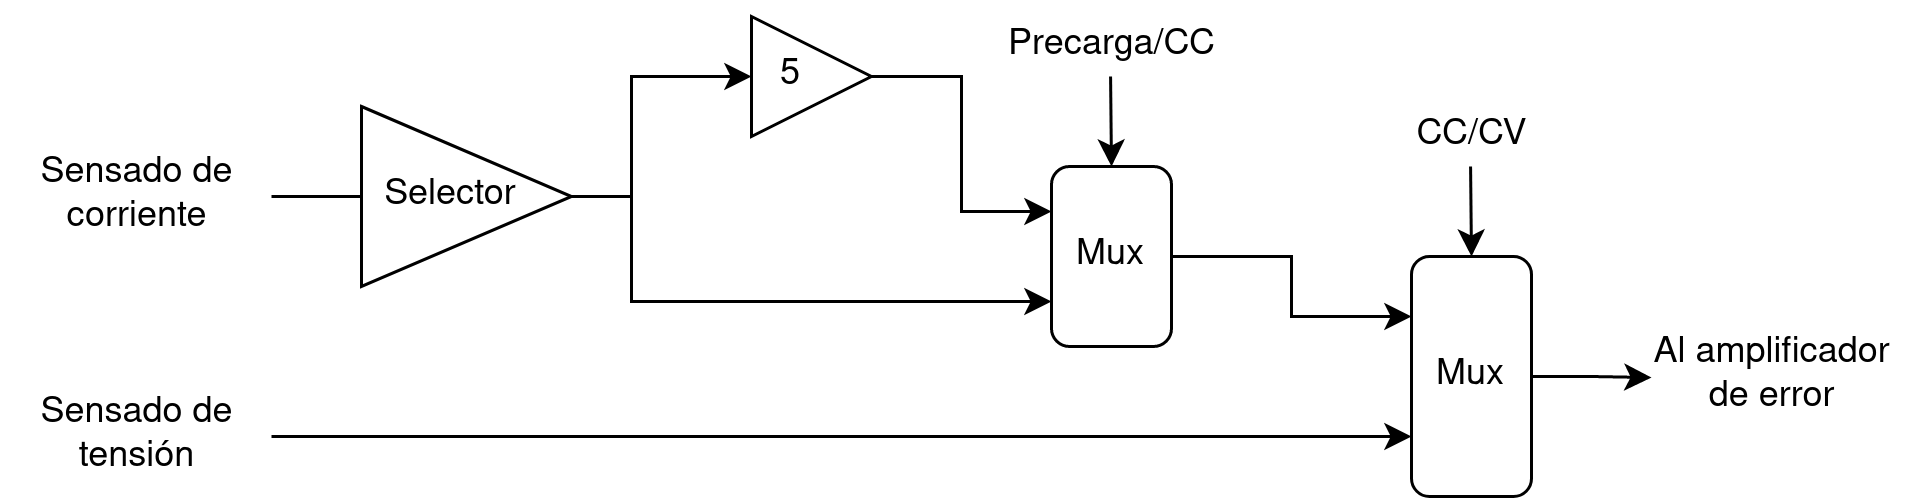
\includegraphics[width=\textwidth]{images/selector.png}
    \caption{Esquema del selector de modo}
    \label{fig:esquema_selector}
\end{figure}

Una vez diseñado el compensador, se procedió a diseñar el circuito de cambio de modo (Precarga, tensión constante y corriente constante).
En la figura \ref{fig:esquema_selector} se puede observar el esquema de este circuito.

Las señales de tensión y corriente están normalizadas con respecto a sus valores nominales.
Un amplificador de ganancia variable actúa como selector de corriente de salida,
modificando la amplitud de la señal de control de dicha variable.
La selección entre el modo de precarga y el modo de corriente constante se hace comparando el nivel de tensión de la batería
con una señal de referencia, siendo el segundo modo activado una vez que la tensión supera los 30V.
El bloque de ganancia 10 tiene como objetivo amplificar la señal de control, ya que la corriente de salida para el modo
de precarga es 10 veces mas chica que la de corriente constante.
% Era realmente 10 veces mas chica? O al final era 5 veces?

La normalización de las señales nombrada anteriormente permite que la selección de la señal del último multiplexor
se haga en base a cual es la mayor de las dos. Esto, visto desde una perspectiva general, permite establecer un límite
tanto de tensión como de corriente de salida, lo cual es importante porque representa la base del método de carga.

Finalmente, para la selección de un controlador para los MOSFETs se tuvieron en cuenta algunos parámetros como
la tensión máxima de entrada, frecuencia de switching y sincronización de las señales,
pero no se logró hallar un controlador adecuado para esta aplicación.
El principal motivo fue que los controladores convencionales generan señales alternadas mediante el método de bootstrapping \cite{hart},
lo cual no sirve para la topología elegida. Esto, combinado con el elevado nivel de tensión en la entrada,
llevó a la búsqueda de otros métodos de control; por eso, se optó por un controlador con transformador aislante para el MOSFET cuyo source no esta a tierra \cite{gatedrivers}. El diagrama de este driver puede observarse en la figura \ref{fig:driver}.

\begin{figure}
    \centering
    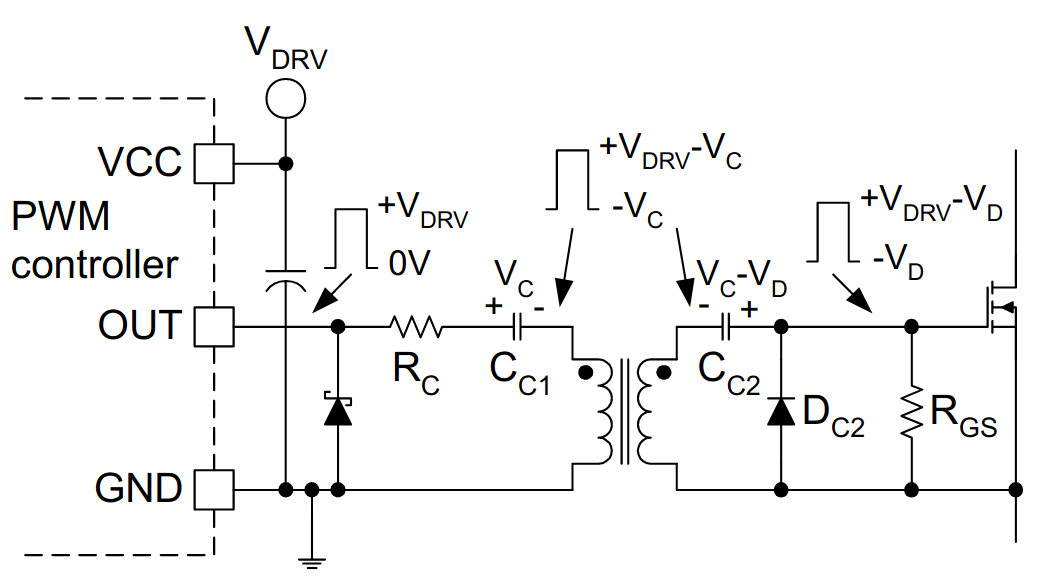
\includegraphics[width=\textwidth]{images/esquema_driver.png}
    \caption{Esquema del controlador del MOSFET de lado alto}
    \label{fig:driver}
\end{figure}

\subsection{Amplificador clase B con transistores complementarios}

Dado que la carga que genera el circuito sobre el TL494 es muy alta, sin esta etapa de amplificación, la forma de onda PWM disminuía su amplitud notablemente y se distorsionaba, lo que causaba que los MOSFETs no se saturaran y aumentaran demasiado su temperatura.
Los resultados obtenidos con la inclusión de esta etapa fueron un incremento notorio en la amplitud y una mejora en la forma de onda de la señal PWM.

La etapa permite acoplar la carga en continua. 
Los transistores utilizados son de potencia y no de señal. 
Cada dispositivo de amplificación conduce durante medio ciclo de la señal de entrada, 
excitándolos mediante el ingreso de corriente por su base.
Se compone de un transistor NPN y otro PNP que se alimentan de forma inversa.
El transistor NPN requiere de una tensión positiva en su colector y 
el transistor PNP requiere de una tensión negativa en su colector.

Ambos funcionan como seguidor por emisor o colector común, con su tensión de alimentación en colector, la señal de excitación en la base y la carga conectada el emisor. 
Su ganancia de tensión es aproximadamente 1.
La topología seguidor por emisor tiene ganancia de corriente $hfe$. 
La corriente que se entrega por la base es $hfe$ veces menor que la que se le entrega a la carga. 
El seguidor presenta una impedancia de entrada es mucho mas alta que su impedancia de salida, de modo que una fuente de señal no tendría que trabajar tan duro.
Esto puede verse en el hecho de que la corriente de base es del orden de 100 veces menos que la corriente de emisor. 
La baja impedancia de salida del seguidor emisor se adapta con una carga de baja impedancia y amortigua la fuente de señal.

Los transistores conducen en base a la tensión $V_{be}$ en sus junturas ya que entre base y emisor existe una juntura PN similar a un diodo. 
Si no se polariza de forma correcta, no circula corriente por su base y en consecuencia tampoco por su colector. 
El transistor NPN conduce corriente en su emisor cuando $V_{be}>0$ mientras que el transistor PNP conduce corriente en su emisor cuando $V_{be}<0$ o $V_{eb}>0$.
Los transistores conducen de forma alternativa: en el semiciclo positivo de la señal conduce el NPN y el PNP se corta y en el semiciclo negativo conduce el PNP y el NPN se corta. 
Cuando la tensión de entrada en la base de ambos transistores es 0 no conduce ningún transistor, es decir, no existe consumo de corriente ni de potencia. 
La $V_{ce}$ de ambos transistores va de $V_{cc}$ a 0.
% Hay muchas frases sueltas en este último parrafo, habría que reordenarlas y unirlas.

\subsection{Driver}

Los MOSFET se encargan de conectar la alimentación con la carga. El IRF840 es un MOSFET de canal N.
Para encenderlo se debe aplicar una tensión positiva entre \textit{gate} y \textit{source}. 
Debido a la configuración de convertidor elegida, se requiere un driver para controlar el MOSFET cuyo terminal de \textit{source} no está a tierra. Se optó por un driver con transformador acoplador ya que provee aislación galvánica entre el circuito de control y el circuito de potencia \cite{gatedrivers}.

Existen 2 posibles configuraciones para un transistor según su posición en el circuito:

\paragraph{Lado bajo} Utiliza comúnmente el MOSFET de canal N. 
El terminal \textit{source} está a tierra y la carga se encuentra entre la alimentación y el terminal \textit{drain}. 
Mientras está encendido le otorga a la carga el camino hacia la tierra y cuando está apagado se sitúa debajo de la misma. 

\paragraph{Lado alto} Utiliza comúnmente el MOSFET de canal P. 
El terminal \textit{drain} se encuentra conectado a la alimentación y el terminal \textit{source} a la carga.\\

% INSERTAR FIGURA DE GOOGLE! <<< Estuve buscando en google y si bien hay varias, estaría mejor poner alguna de un libro. Pero el mohan y el rashid no tienen ninguna

Para controlar MOSFETs de lado alto se puede utilizar un circuito integrado o un transformador. 
Los circuitos integrados, si bien son más pequeños y ocupan menor espacio en las placas, 
poseen tiempos significativos de encendido y apagado. 
El transformador es de un tamaño mucho mayor, requiere de un diseño apropiado y de componentes adicionales,
pero sus tiempos de encendido y apagado son despreciables y permite operar con diferencias de tensión más elevadas.

Los transformadores poseen al menos 2 bobinados acoplados magnéticamente, 
lo cual permite generar aislación entre el circuito primario y secundario. 
La relación de vueltas entre los mismos permite modificar la tensión de salida obtenida. 
Los transformadores manejan muy poca potencia promedio, pero entregan altos picos de corriente en el encendido y apagado.

Si bien el transformador ideal no almacena energía, los transformadores reales 
almacenan una pequeña cantidad de energía entre los bobinados y los posibles huecos de aire presentes en el mismo. 
Esto se representa mediante una inductancia magnetizante. 
Una pequeña inductancia minimiza la energía almacenada permitiendo aumentar la eficiencia y disminuye los retrasos de tiempo. 

Para cumplir con la ley de Faraday, la tensión en la bobina del transformador debe ser nula en una parte del período, 
por lo cual cualquier pequeña señal de continua puede hacer saturar al núcleo. 
La saturación limita el producto volt-segundo aplicado a través de los devanados. 
Su valor máximo se da en la peor condición de funcionamiento con el ciclo de trabajo máximo y la tensión de entrada máxima simultáneamente. 

Como el convertidor forward trabaja sólo en el primer cuadrante del plano B-H, una gran parte del período de switching debe reservarse para restaurar el núcleo de la potencia del transformador. 
Esto limita la relación de trabajo del transformador, pero no suele ser un problema ya que 
el transformador debe estar acoplado a corriente alterna y por lo tanto funciona con magnetización bidireccional. 

%Perá, acá estamos mezclando muchisimo el driver del mosfet con el resto del conversor. Esta seccion para cual de los 2 es?
La figura \ref{fig:driver} muestra el circuito básico del driver mediante un transformador.

A continuación se detalla información relevante de cada componente: 

\paragraph{Entrada single-ended} 

Este driver en particular está diseñado para convertir la salida de un extremo de un controlador PWM a una señal de doble extremo. % Traduccion de mierda

\paragraph{Capacitor de acoplamiento $C_{C_1}$}

Para evitar la componente continua se coloca un capacitor de acoplamiento en serie con el bobinado primario, 
evitando la saturación del núcleo. La tensión sobre el mismo resulta: 

$$ V_{cc_1}=D\cdot V_{drv} $$

En base al máximo ripple de tensión permitido y la carga que atraviesa a los capacitores de acoplamiento en estado estacionario:

%INSERTAR FÓRMULA DE CC1
$$ C_{C_1}=\frac{Q_G}{\Delta V_{C_1}}+\frac{(V_{drv}-V_{dc2,fw})D}{\Delta V_CR_{gs}f_{drv}}+\frac{V_{drv}(D^2-D^3)}{\Delta V_{C_1}\cdot4\cdot L_mf_{drv}^2} $$

Para este capacitor, el ripple tiene una componente relacionada a la carga del MOSFET, 
otra relacionada con la corriente que pasa por la resistencia entre \textit{gate} y \textit{source} 
y una última componente relacionada a la corriente de la inductancia magnetizante. 
La capacidad es máxima para un ciclo de trabajo determinado definido por los parámetros de diseño 
y los valores de los componentes y se obtiene derivando a la expresión en función del ciclo. 

Constante de tiempo de la tensión en el capacitor de acoplamiento:

$$ \tau=R_{gs}C_{C_1} $$

Para anchos pulsos del ciclo de trabajo, se requieren de componentes adicionales 
en el secundario del transformador para proveer de la tensión correcta al \textit{gate}. 
La tensión a través del capacitor de acoplamiento se incrementa de forma proporcional al pulso. 
La tensión negativa durante el tiempo que está apagado aumenta y la tensión positiva durante el tiempo que está encendido disminuye. 

%INSERTAR FORMA DE ONDA SOBRE EL CAPACITOR (SE SACA DEL ESQUEMÁTICO DADO)

\paragraph{Resistencia de amortiguamiento $R_C$}

Cambios repentinos en el ciclo de trabajo excitan a la red LC compuesta por el capacitor de acoplamiento 
y la inductancia magnetizante, provocando resonancias indeseadas en la tensión sobre el capacitor. 
Esta resistencia de bajo valor en serie con el capacitor de acoplamiento permite amortiguar las resonancias. 

$$ R_c\geq2\cdot\sqrt{\frac{L_m}{C_{C_1}}} $$

Si la resistencia es muy grande, genera una sobre amortiguación que limita la corriente que ingresa al terminal \textit{gate} y disminuye la frecuencia de switching. 
Si la resistencia es muy chica, las resonancias provocadas generan una tensión entre \textit{gate} y \textit{source} muy elevada.

\paragraph{Resistencia de carga entre \textit{gate} y \textit{source} $R_{gs}$}

Es una resistencia de pull down que pone a tierra el terminal \textit{gate} al alimentar el circuito, manteniendo al MOSFET apagado durante el inicio. 
Además le provee de un camino para la corriente que circula por el capacitor de acoplamiento, 
permitiendo establecer la tensión necesaria sobre el mismo y que en cada ciclo de switching 
la misma carga del \textit{gate} sea entregada y removida a través del capacitor. 

\paragraph{Diodo Schottky}

Debido a la componente de corriente de la inductancia magnetizante, la salida debe manejar corriente de forma bidireccional. 
Por ello se requiere un diodo Schottky a la entrada. 
El mismo puede evitarse aumentando la componente de corriente resistiva para contrarrestar a la componente de la inductancia magnetizante. 

\paragraph{Capacitor de acoplamiento $C_{C_2}$}

Se agrega un segundo capacitor de acoplamiento que permite restaurar a los niveles originales de tensión. 
El agregado opcional de un diodo zener en serie permite incrementar aún más la tensión negativa durante el apagado. 

En base al máximo ripple de tensión permitido y la carga que atraviesa a los capacitores de acoplamiento en estado estacionario:

% INSERTAR FÓRMULA DE CC2 
% CORREGIR DE LA FÓRMULA: ES VDRV Y NO VDRC
$$ C_{C_2}=\frac{Q_G}{\Delta V_{C_2}}+\frac{(V_{drv}-V_{dc2,fw})D_{max}}{\Delta V_{C_2}R_{gs}f_{drv}} $$

Para este capacitor, el ripple tiene una componente relacionada a la carga del MOSFET 
y otra relacionada con la corriente que pasa por la resistencia entre \textit{gate} y \textit{source}. 
La capacidad es máxima cuando el ciclo de trabajo es máximo. 

\paragraph{Diodo clamp}

%Evita sobre tensiones. <<< Esto era así? No evitaba tension negativa a la salida?
Mantiene la tensión entre \textit{gate} y \textit{source} por arriba de $-V_\gamma$.\\

\subsubsection{Diseño del transformador}

Su diseño es similar a un transformador de potencia. 
Su función es transmitir el pulso de accionamiento de puerta referenciado a tierra a través de grandes diferencias de potencial para adaptarse a las implementaciones de accionamiento flotante. Para hacerlo maneja muy poca potencia pero requiere de elevados picos de corriente. 

Su relación será 1:1 ya que no se requiere cambiar el nivel de tensión.
Está controlado por un ancho de pulso variable y de amplitud constante,
acoplado a CA y la inductancia de magnetización ve un pulso de amplitud variable.
Operan en el primer y tercer cuadrante del plano B-H.

Primero se selecciona el núcleo. En base a la disponibilidad se elige el E25. 
El material del núcleo es ferrita de alta permeabilidad para maximizar el valor de 
la inductancia de magnetización y, en consecuencia, reducir la corriente de magnetización.

El número de vueltas del primario se calcula como: 

%INSERTAR FÓRMULA DEL NÚMERO DE VUELTAS JUNTO A LA DESCRIPCIÓN DE CADA variable


Primero se halla el numerador con:

%INSERTAR IMÁGEN 36: Gate-Drive Transformer Volt-second Product vs. Duty Ratio

Para un circuito acoplado de CA, el peor de los casos es $D=0.5$, 
mientras que el acoplamiento directo alcanza el valor pico de voltios por segundo en la máxima relación de trabajo operativa. 
Curiosamente, el acoplamiento de CA reduce el producto volt-segundo de estado estacionario máximo en un factor de cuatro debido a que, 
en relaciones de trabajo grandes, el voltaje del transformador se reduce proporcionalmente debido al voltaje que 
se desarrolla a través del capacitor de acoplamiento.
%Delta B: valor pico a pico del cambio en el flujo que se produce durante la duración del pulso. 

Es mucho más difícil calcular $\Delta B$ en la ecuación $N_p$. 
La razón es el desplazamiento del flujo durante el funcionamiento transitorio. 
Cuando el voltaje de entrada o la carga cambian rápidamente, el controlador PWM ajusta la relación de trabajo en consecuencia. 
Es bastante difícil deducir el resultado cuantitativo exacto de la caminata de flujo. 
Depende de la respuesta del lazo de control y de la constante de tiempo de la red de acoplamiento cuando está presente. 
En general, una respuesta de bucle más lenta y una constante de tiempo más rápida tienden a reducir el desplazamiento de flujo. 
Para la mayoría de los diseños, es deseable un margen de tres a uno entre la densidad de flujo de saturación 
y el valor de flujo máximo en el peor de los casos de operación en estado estable para cubrir la operación transitoria.

\subsection{Snubber} \label{subsec:oscilaciones}

Un circuito snubber o de amortiguación es una red RC que permite eliminar ruido de alta frecuencia que existe en los nodos de los transistores.
Hasta ahora se ha analizado el convertidor forward sin tener en cuenta los elementos parásitos asociados a cada componente. 
Algunos ejemplos de estos son la resistencia serie equivalente e inductancia serie equivalente de los capacitores, 
la capacidad parásita de los transistores o la resistencia e inductancia parásita de las conexiones realizadas. 
La energía acumulada en las inductancias parásitas mientras los transistores conmutan provoca una resonancia con el capacitor de filtrado en la entrada. 
La red snubber conforma un camino de baja impedancia para el drenaje de esta energía. 
Valores pequeños de estos elementos parásitos generan resonancias del orden de los MHz. 

\subsubsection{Funcionamiento}

La energía acumulada en las inductancias parásitas mientras los transistores están encendidos se almacena como energía electroestática en el capacitor de la red snubber $C_{snb}$. 
Cuando los transistores conducen, su tensión se eleva hasta $V_{in}$, la energía almacenada en el capacitor es: 

$$ E=0.5\times C_{snb}V_{in}^{2} $$

La carga eléctrica del capacitor luego de su carga es:

$$ Q=C_{snb}V_{in} $$

La potencia suministrada por la fuente de entrada en cada ciclo es:

$$ V_{in}Q=C_{snb}V_{in}^{2} $$

Las pérdidas en la resistencia $R_{sbn}$ resultan:

$$ P_{R_{snb}}=C_{snb}V_{in}^{2}f_{sw} $$

Durante la carga mitad de esta potencia se consume en la resistencia $R_{snb}$ por efecto Joule y la otra mitad se almacena en el capacitor $C_{snb}$. 
Cuando los transistores no conducen, su tensión disminuye hasta $0V$, toda la energía almacenada se descarga y es consumida en la resistencia de amortiguamiento $R_{snb}$.
Cuando se descarga, mitad de la energía almacenada se convierte en calor en la resistencia $R_{snb}$. 
El análisis supone que el tiempo de carga y descarga es mucho más grande que la constante de tiempo RC. 

\subsubsection{Procedimiento para el cálculo de los componentes}

\begin{enumerate}
    \item Con el osciloscopio se mide la frecuencia de la oscilación en la tensión del transistor Vds. $f_{r}=1.27MHz$ %Era esa?
    \item Se conecta un capacitor entre \textit{drain} y \textit{source} con una capacidad $C_{p_{0}}$ tal que la frecuencia de la oscilación disminuya a la mitad. $C_{p_{0}}=$
    \item La frecuencia de resonancia en una red LC está dada por
    $$ w=\frac{1}{\sqrt{LC}} $$
    Con la configuración actual, 
    $$ f_{r}=\frac{1}{2\pi\sqrt{L_{p}(C_{p_{2}}+C_{p_{0}})}} $$
    Para lograr que dicha frecuencia disminuya a la mitad se necesita una capacitancia total que sea cuatro veces la capacitancia parásita con la que se comenzó.
    Por lo tanto, la capacidad parásita del circuito resulta un tercio de la capacidad agregada. $C_{p_{2}} = \frac{C_{p_{0}}}{3}$
    \item Teniendo la capacidad parásita del circuito Cp2 y la frecuencia de la oscilación original se puede calcular la inductancia parásita del circuito:
    $$ L_{p}=\frac{1}{(2\pi f_{r})^{2}*C_{p_{2}}} $$
    \item La impedancia característica de los elementos parásitos resulta:
    $$ Z_{0}=\sqrt{\frac{L_p}{C_{p_2}}} $$
    \item El valor óptimo para la $R_{snb}$ es aproximadamente igual a la impedancia característica. Debe ser mayor o igual a esta última. Un valor muy alto puede permitir un pico propio de la oscilación y un valor más bajo permite una corriente más elevada, resultando en un sobrecalentamiento.
    \item Se elige una Csnb que sea igual o hasta 4 veces superior a la capacidad parásita del circuito. $C_{p_2}\leq C_{snb}\leq 4C_{p_2}$
    \item Se calcula la potencia disipada en Rsnb y se utiliza una resistencia cuya potencia máxima sea el doble que la disipada.
    $$ P_{R_{snb}}=C_{snb}V_{in}^2f_{sw} $$
    \item Se agrega un capacitor de \textit{bypass} de 0.1uF para amortiguar la inductancia del MOSFET de lado alto.     
\end{enumerate}